% \documentclass[ba,preprint]{imsart}% use this for supplement article
\documentclass[ba]{imsart}

%% Packages
\RequirePackage{amsthm,amsmath,amsfonts,amssymb}
\RequirePackage[numbers]{natbib}
%\RequirePackage[authoryear]{natbib}%% uncomment this for author-year citations
\RequirePackage[colorlinks,citecolor=blue,urlcolor=blue,backref=page,backref=page]{hyperref}
\RequirePackage{graphicx}


%%%%%%%%%%%packages added by Spencer%%%%%%%%%%%%%
\usepackage{booktabs} %for the table in the analysis section
\usepackage{enumerate} %for the short algorithm
\usepackage{subfigure} %for making plots with multiple images
\usepackage{tabularx} %for the spacing in tabular
\usepackage{newtxmath} %for making indicator function
\usepackage{changepage} %for adjusting the margins
%%%%%%%%%%%%%%%%%%%%%%%%%%%%%%%%%%%%%%%%%%%%%%%%%

\pubyear{2024}
\arxiv{2010.00000}
\volume{TBA}
\issue{TBA}
\firstpage{1}
\lastpage{1}

\startlocaldefs
%%%%%%%%%%%%%%%%%%%%%%%%%%%%%%%%%%%%%%%%%%%%%%
%%                                          %%
%% Uncomment next line to change            %%
%% the type of equation numbering           %%
%%                                          %%
%%%%%%%%%%%%%%%%%%%%%%%%%%%%%%%%%%%%%%%%%%%%%%
%\numberwithin{equation}{section}
%%%%%%%%%%%%%%%%%%%%%%%%%%%%%%%%%%%%%%%%%%%%%%
%%                                          %%
%% For Axiom, Claim, Corollary, Hypothesis, %%
%% Lemma, Theorem, Proposition              %%
%% use \theoremstyle{plain}                 %%
%%                                          %%
%%%%%%%%%%%%%%%%%%%%%%%%%%%%%%%%%%%%%%%%%%%%%%
\theoremstyle{plain}
\newtheorem{axiom}{Axiom}
\newtheorem{claim}[axiom]{Claim}
\newtheorem{theorem}{Theorem}[section]
\newtheorem{lemma}[theorem]{Lemma}
%%%%%%%%%%%%%%%%%%%%%%%%%%%%%%%%%%%%%%%%%%%%%%
%%                                          %%
%% For Assumption, Definition, Example,     %%
%% Notation, Property, Remark, Fact         %%
%% use \theoremstyle{definition}            %%
%%                                          %%
%%%%%%%%%%%%%%%%%%%%%%%%%%%%%%%%%%%%%%%%%%%%%%
\theoremstyle{definition}
\newtheorem{definition}[theorem]{Definition}
\newtheorem*{example}{Example}
\newtheorem*{fact}{Fact}
%%%%%%%%%%%%%%%%%%%%%%%%%%%%%%%%%%%%%%%%%%%%%%
%%                                          %%
%% For Case use \theoremstyle{remark}       %%
%%                                          %%
%%%%%%%%%%%%%%%%%%%%%%%%%%%%%%%%%%%%%%%%%%%%%%
\theoremstyle{remark}
\newtheorem{case}{Case}
%%%%%%%%%%%%%%%%%%%%%%%%%%%%%%%%%%%%%%%%%%%%%%
%% Please put your definitions here:        %%
%%%%%%%%%%%%%%%%%%%%%%%%%%%%%%%%%%%%%%%%%%%%%%
\endlocaldefs

\begin{document}


\begin{supplement}
\renewcommand{\thesection}{\Alph{section}}

\section{Additional plots for ILI \& Hospitalization data for select regions,
         results from simulation study, and 2023-24 flu analysis}

Figure \ref{fig:ili_vs_week} shows ILI data all 50 states in the US. 
The plots include the ILI data for all seasons from 2010 to 2023 in grey, 
and the black line is the per week ILI average over seasons. 
The patterns in the individual states are similar to the national 
level plots in that the ILI rises in the fall and winter until it peaks 
and descends as the spring and summer progress. 
It can also be seen that neighboring states tend to have similar ILI levels.
At nearly all states, the ILI typically peaks, either locally or globally, 
at or near 
week 22. 

 \begin{figure}[hbt!]
    \centering
    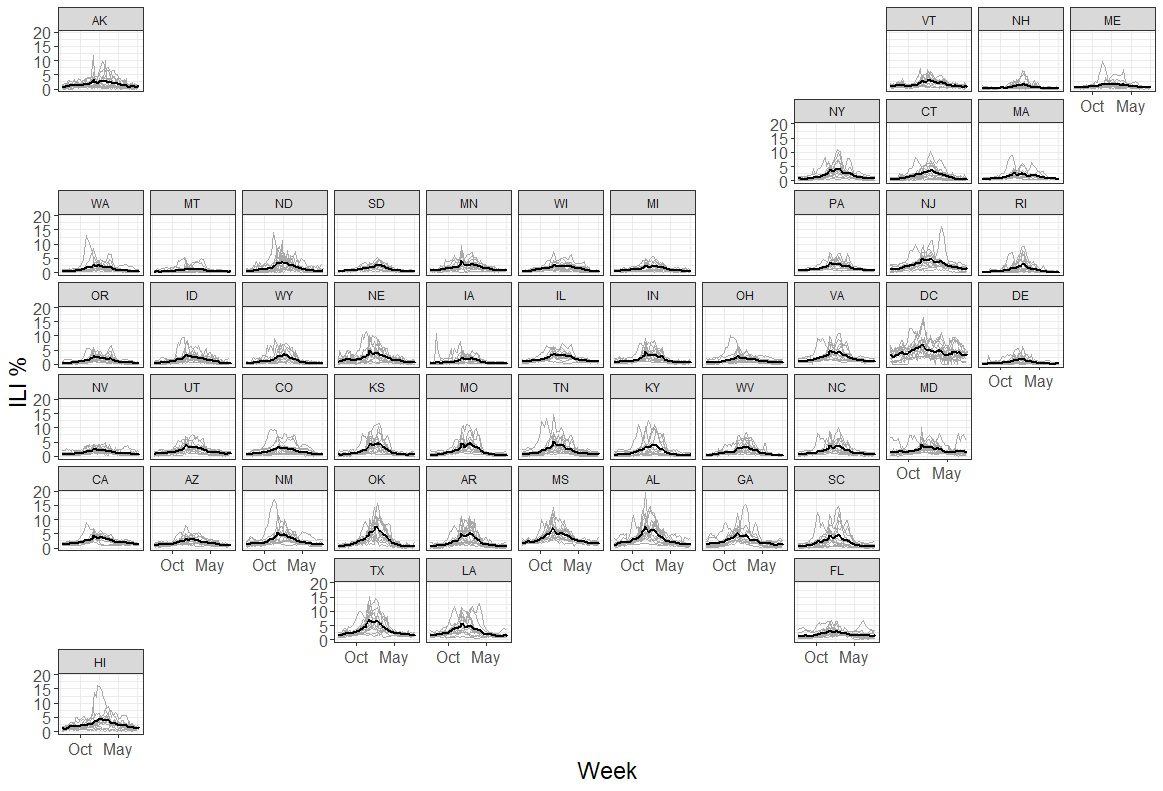
\includegraphics[scale=.45]{Images/ili_vs_week.png}
    \caption{Percentage of outpatient visits with an influenza-like illness 
    (ILI) for the 50 US states seasons 2010 to 2023. Week 1 is the first week 
    of August of the year the flu season begins and the last week of the 
    season is the last week of July of the following year.
     Plots include lines for ILI\% from the 2010 flu season to 2023 (grey) 
     and for the weekly ILI averaged over all seasons (black).}
    \label{fig:ili_vs_week}
\end{figure}


Figure \ref{fig:hosp_vs_week} shows the 2022 and 2023 weekly hospitalizations 
for the 50 US states. Similar to the US national data, 
the state peaks in 2022 came early compared to the peak of 2023. 
This figure shows hospitalization levels may similar for neighboring states,
but also that state population plays a role in the number of hospiatlizations.
Comparing figures 
\ref{fig:ili_vs_week} and \ref{fig:hosp_vs_week} shows that ILI and 
hospitalizations share the similar pattern of increasing to a peak in the 
winter and decreasing thereafter. 

\begin{figure}[hbt!]
    \centering
    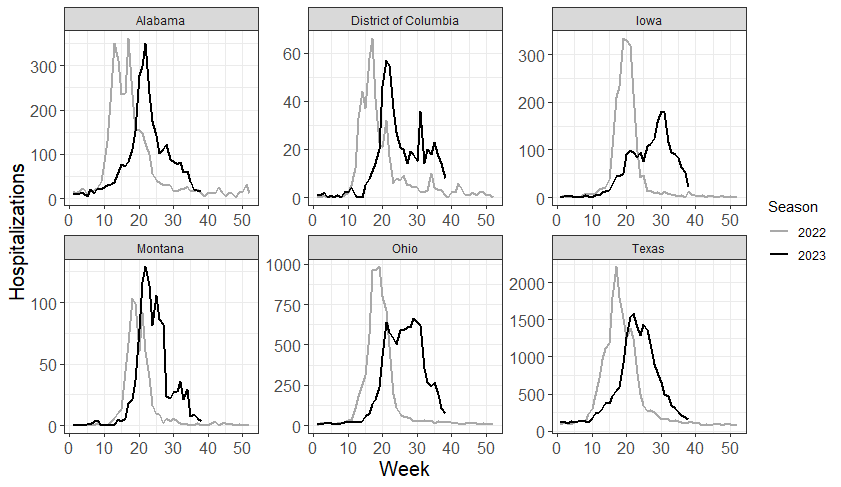
\includegraphics[scale=.5]{Images/hosp_vs_week.png}
    \caption{Weekly hospitalization counts for the 50 US states for the 2022 
    (grey) and 2023 (black) flu seasons.}
    \label{fig:hosp_vs_week}
\end{figure}













\section{Prior distributions} \label{app:B_prior}

The prior distributions under the SIR model are in (\ref{eq:sir_prior}).
Because we set $S_{0s} = 0.9$, prior distributions were assigned only to
$I_{0s}$, $\beta_s$ and $\rho_s$, recalling the parameter for the recovery
rate $\delta_s = \rho_s \beta_s$. Here $\vmathbb{1}_{A}$ represents the
indicator function for values within the set $A$.

\begin{equation}
\begin{aligned}
    \label{eq:sir_prior}
        I_{0s} &\sim N(0.005, 0.03) \vmathbb{1}_{(0, .1)} \\
        \beta_s &\sim N^+(0.8, 0.3) \\
        \rho_s &\sim N^+(0.68, 0.08)
\end{aligned}
\end{equation}
For the ASG model, the MLE 
$\hat{\theta}_s = (\hat{\lambda}_s, \hat{\eta}_s, \hat{\mu}_s, \hat{\sigma}_{1s}^2, \hat{\sigma}_{2s}^2)$ 
was calculated. % and $\hat{\lambda}_s$ was accepted as a fixed value. 
These estimates were used as starting values for posterior sampling. 
The transformation 
$T(\theta_s) = (\lambda_s, \text{log}(\eta_s), \mu_s, \text{log}(\sigma_{1s}^2), \text{log}(\sigma_{2s}^2))$ 
was made, and a prior distribution was assigned to $T(\theta_s)$.
The prior distributions for the ILI model under the ASG function 
without discrepancy are shown 
in (\ref{eq:ili_prior}). These are slightly informative priors because for 
most parameters we have an idea what reasonable values may be. Here 
$m = (-4.5, 0.3, 23, 3.69, 4.7)$ and $C = \text{diag}(0.3, 0.2, 5, 2, 2)$
where $\text{diag}(\cdot)$ 
is the diagonal matrix for the given entries. When modeling ASG with 
discrepancy, the first entry in $m$ was replaced with $\hat{\lambda}$ the 
mean over seasons of MLEs for that parameter, and in the matrix $C$
the first diagonal 
variance parameter of $0.3$ was replaced with $0.01$. This was done to alleviate
the identifiability issues of $\lambda_s$ that are indtroduced when including 
discrepancy in the ILI model.


\begin{equation}
\begin{aligned}
\label{eq:ili_prior}
                T(\theta_s) &\overset{ind}{\sim} MVN(\theta, \Sigma) \\
                T(\theta) &\overset{ind}{\sim} MVN(m, C)\\
                \Sigma &= \text{diag}(\zeta^2_1,...,\zeta^2_4) \\
                \zeta_i &\overset{ind}{\sim} N^+(0,4^2)
\end{aligned}
\end{equation}
Parameters shared by both the SIR and ASG models are the scale parameter 
$\kappa_s$ and the discrepancy parameters $\sigma_{\gamma}^2$ and 
$\sigma_{\gamma_W}^2$. These priors are in (\ref{eq:shared_ili_priors}). 

\begin{equation}
\begin{aligned}
    \label{eq:shared_ili_priors}
        \kappa_s &\overset{ind}{\sim} N^+(0, 10,000^2) \\
        \sigma_{\gamma}^2 &\sim N^+(0, .02^2) \\
        \sigma_{\gamma_W}^2 &\sim N^+(\hat{\sigma}_W^2, 1^2) \\
        \sigma_{\upsilon_{s,w}} &\sim N^+(0, .1^2)
\end{aligned}
\end{equation}
Because of the limited information for estimating $\sigma_{\gamma_W}^2$, 
we selected an informative prior distribution by first estimating  
$\hat{\sigma}_{\gamma_W}^2$. This was estimated for a given state by first 
calculating the MLE for $\theta_s$. 
% We set the likelihood function as $\mathcal{L}(\theta_s) = \prod_{w = 1}^W f_{\theta_s}(w)$ and  calculated $\hat{\theta}_s$ where $\label{eq:theta_hat}
%     \hat{\theta}_s = \underset{\theta_s}{\mathrm{argmin}} \, \mathcal{L}(\theta_s)$.
$\widehat{ILI}_{s,w}$ was then predicted such that 
$\text{logit}(\widehat{ILI}_{s,W}) = f_{\hat{\theta}_s}(W)$ for each season. 
Then $\hat{\sigma}_{\gamma_W}^2$ was calculated as the estimated variance over 
seasons of the differences 
$\text{logit}(\widehat{ILI}_{s,w}) - \text{logit}(ILI_{s,w})$. 
When $f_{\theta_s}(w)$ was the SIR function, $\widehat{\theta}_s$ was 
calculated using the \texttt{mle2} function in the \texttt{bblme} package 
\cite[]{bolker2023bblme} and the \texttt{ode} function in the \texttt{deSolve} 
package \cite[]{soetaert2010desolve} function in \texttt{R}. Where the ASG 
function was used,  $\hat{\theta}_s$ was calculated using the \texttt{optim} 
function.
The prior for the hospitalization models are in (\ref{eq:shared_hosp_priors}).

\begin{equation}
\begin{aligned}
\label{eq:shared_hosp_priors}
        \alpha_{0s} &\overset{ind}{\sim} N(0, 5^2)\\
        \alpha_{1s} &\overset{ind}{\sim} N(0, 5^2)\\
        \alpha_{2s} &\overset{ind}{\sim} N(0, 5^2) \\
        \phi &\sim N(0, .4)\vmathbb{1}_{(-1,1)} \\
        \sigma_{\epsilon_s} &\overset{ind}{\sim} N^+(0, 4^2) \\
        \omega_s &\overset{ind}{\sim} N^+(0, 15^2)
\end{aligned}
\end{equation}





\section{Posterior distribution plots for select parameters}
\label{app:C_post}

The figures in this section show 95\% credible intervals for model parameters 
under the several modeling schemes along with the prior distributions assigned
to the parameters. Figure \ref{fig:posterior_theta_sir} is for parameters 
unique to the SIR ILI model. Figure \ref{fig:posterior_theta}  
show parameters unique to the ASG models. 
Figure \ref{fig:sir_asg_shared} is for parameters shared by SIR and ASG 
models, including parameters used for modeling discrepancy. Figures 
\ref{fig:hosp_lin_params} and \ref{fig:hosp_nus_param} are for parameters 
used in hospitalization modeling.


\begin{figure}[hbt!]
    \centering
    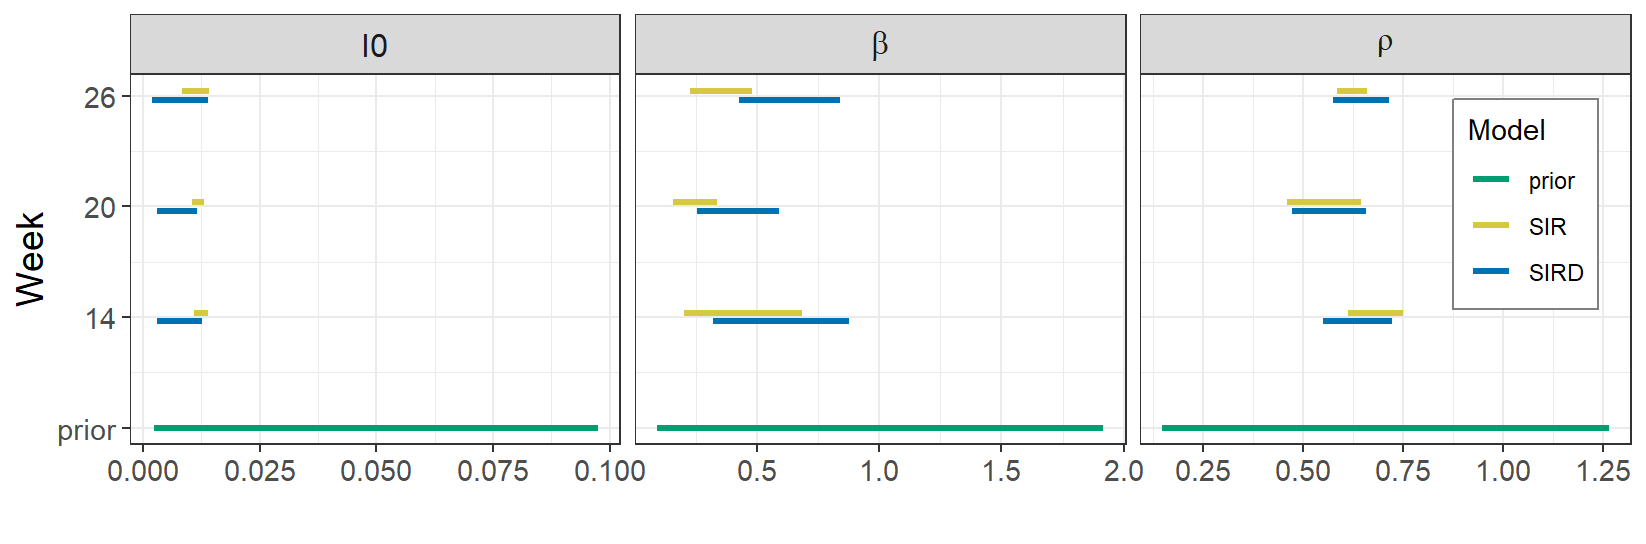
\includegraphics[scale=.6]{Images/posterior_sir.png}
    \caption{Posterior 95\% credible intervals from ILI model for 
    parameters of SIR differential equations. Shown are intervals 
    from the US model of ILI for weeks 14, 20, and 26 and coloured by 
    SIR and SIRD
    models and the assigned prior distributions.}
    \label{fig:posterior_theta_sir}
\end{figure}

\begin{figure}[hbt!]
    \centering
    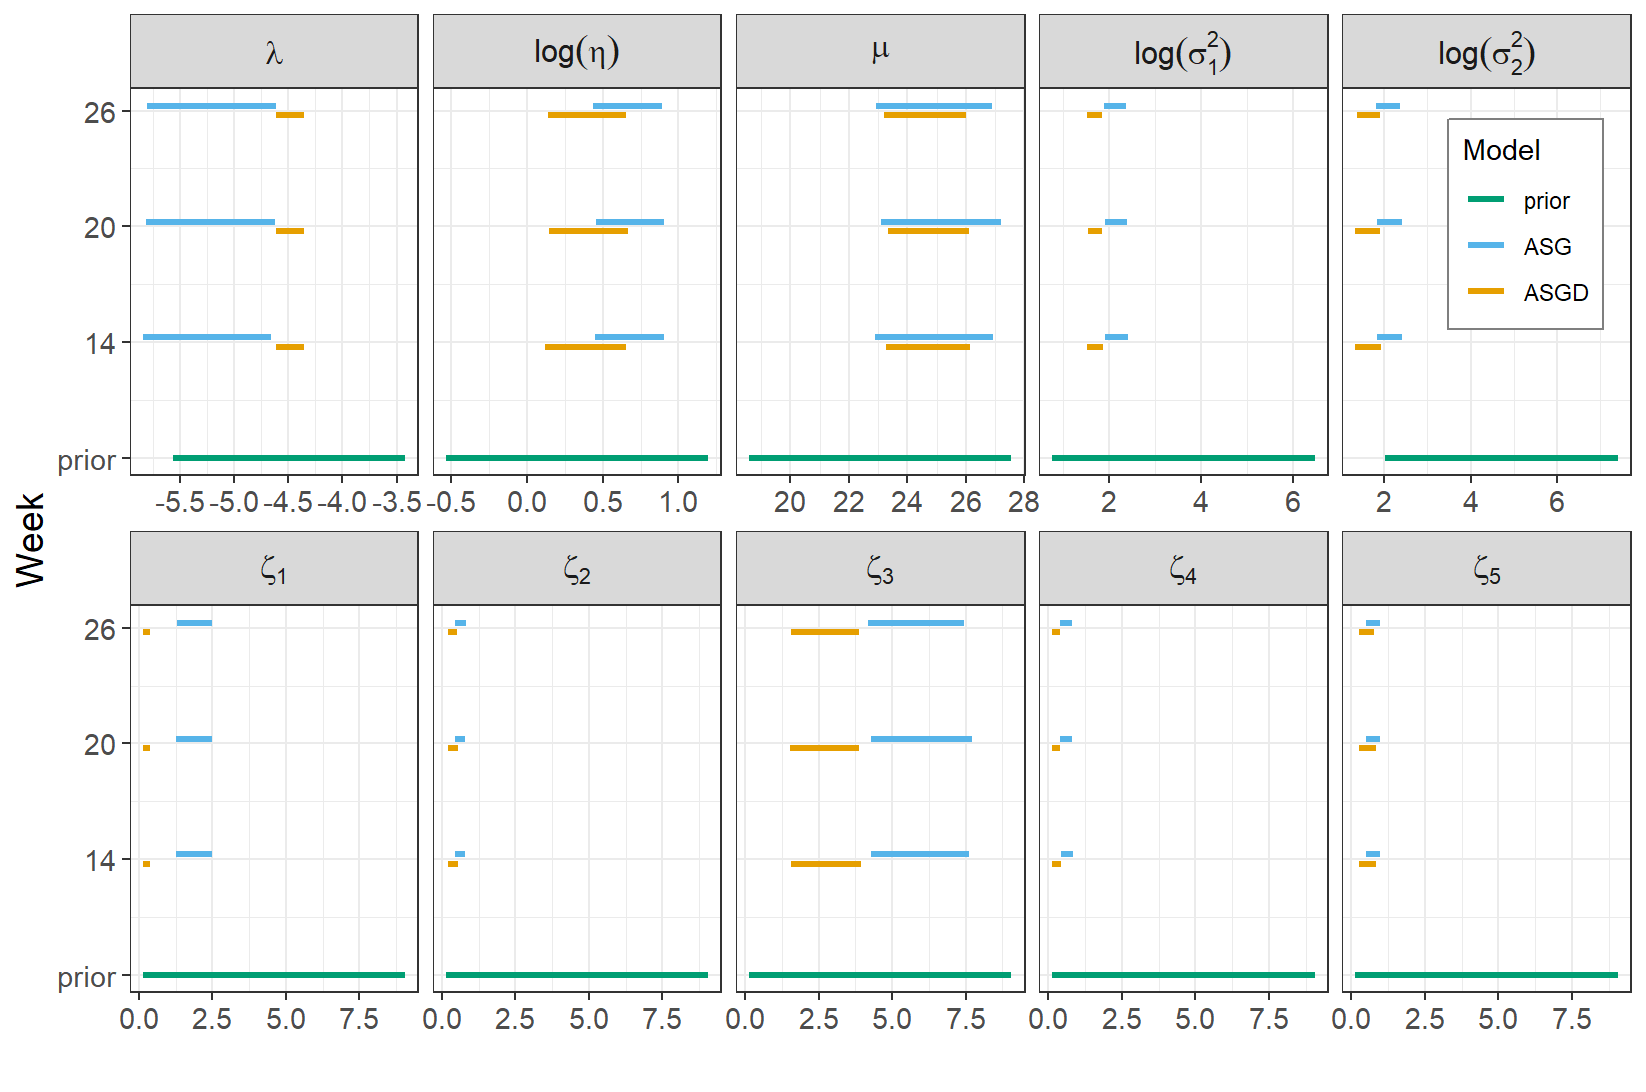
\includegraphics[scale=.6]{Images/posterior_asg.png}
    \caption{Posterior 95\% credible intervals from ILI model for parameters of 
    ASG function. Shown are intervals from the US model of ILI for weeks 14, 
    20, and 26 and coloured by ASG and ASGD models and the assigned 
    prior distributions.}
    \label{fig:posterior_theta}
\end{figure}



\begin{figure}[hbt!]
\centering
  \centering
  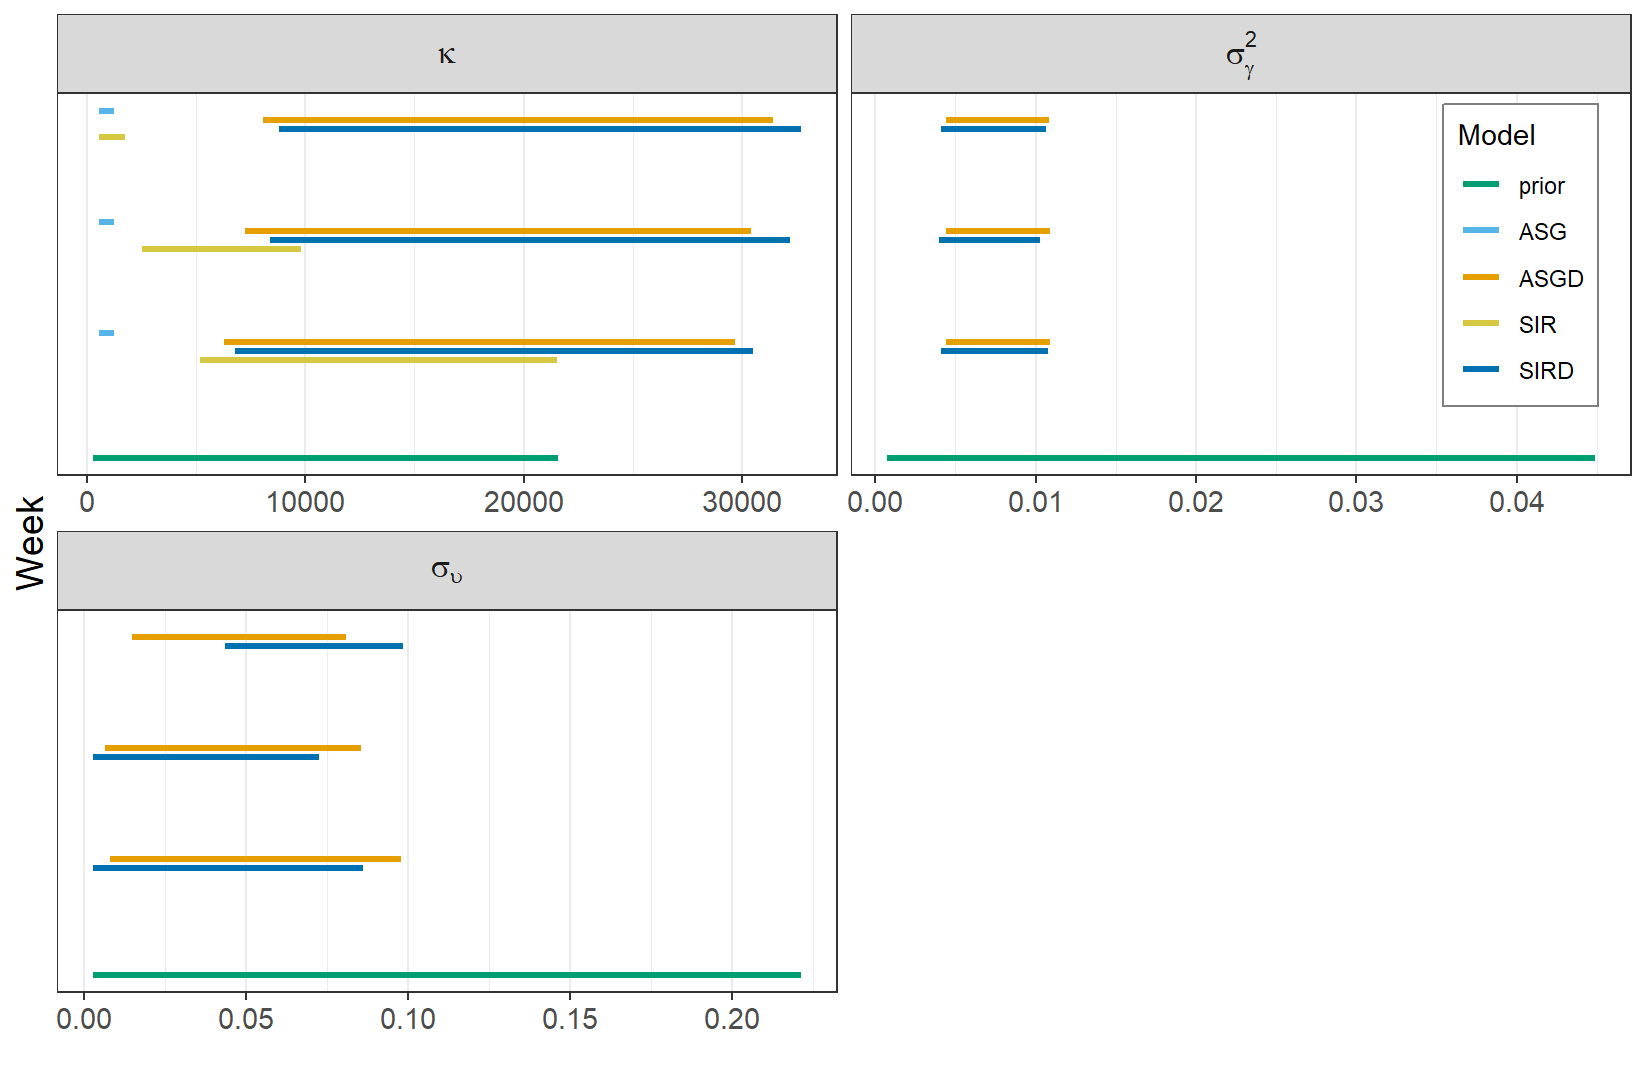
\includegraphics[width=.95\linewidth]{Images/posterior_comb.png}
  % \caption{95\% posterior credible intervals from ILI model for scale parameter of the model distribution. Shown are intervals from the US model of ILI for weeks 14, 20, and 26. The blue is from the SIR model, purple from SIRD, red from ASG and yellow from ASGD. The green interval is the 95\% interval of the prior distribution.}
  % \label{fig:sub1}
\caption{Posterior 95\% credible intervals from ILI model for scale 
parameter $\kappa_s$. 
Blue is from the SIR model, purple from SIRD, 
red from ASG and yellow from ASGD (left).  
Posterior 95\% credible intervals from ILI model for scale parameter of 
modeled discrepancy $\sigma_{\gamma}$ (right). Shown are intervals from the 
US model of ILI for weeks 14, 20, and 26. Blue is from the SIRD model and red 
from ASGD. The green interval is the 95\% interval of the prior distribution.}
\label{fig:sir_asg_shared}
\end{figure}








\begin{figure}[hbt!]
\centering
\begin{subfigure}
  \centering
  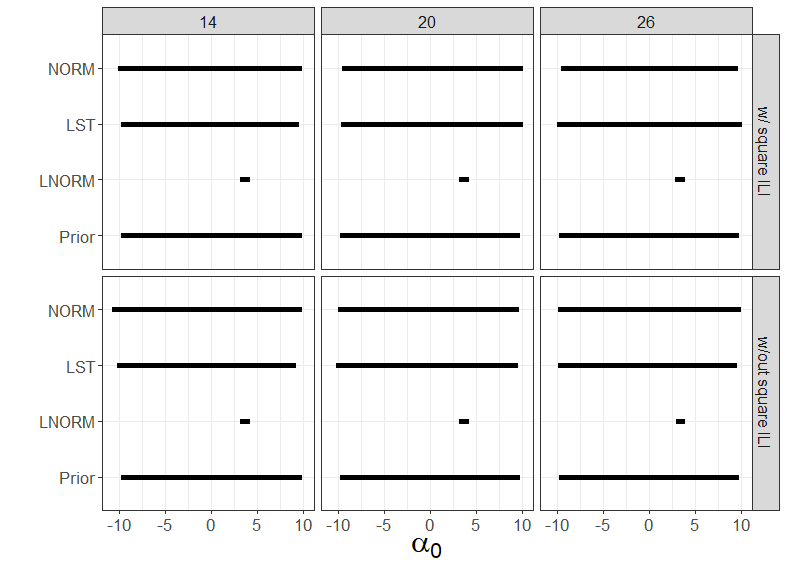
\includegraphics[width=.49\linewidth]{Images/alpha0_post.png}
\end{subfigure}%
\begin{subfigure}
  \centering
  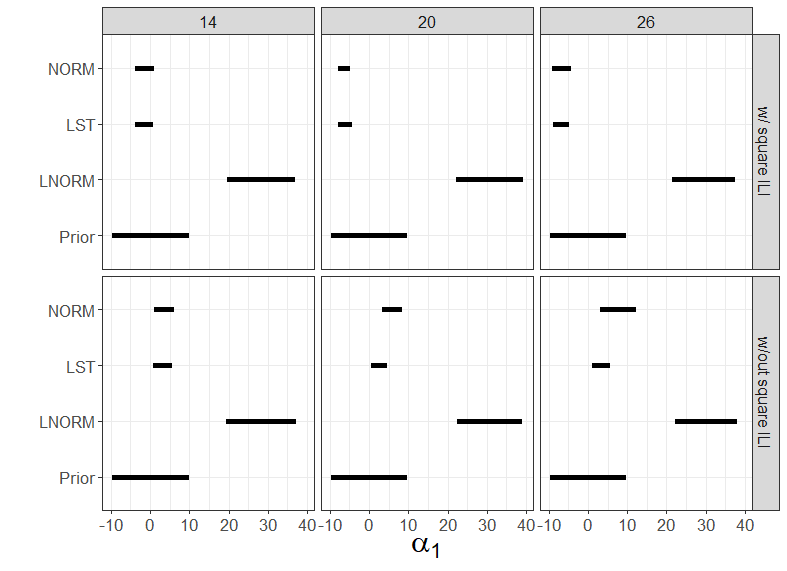
\includegraphics[width=.49\linewidth]{Images/alpha1_post.png}
\end{subfigure}
\begin{subfigure}
  \centering
  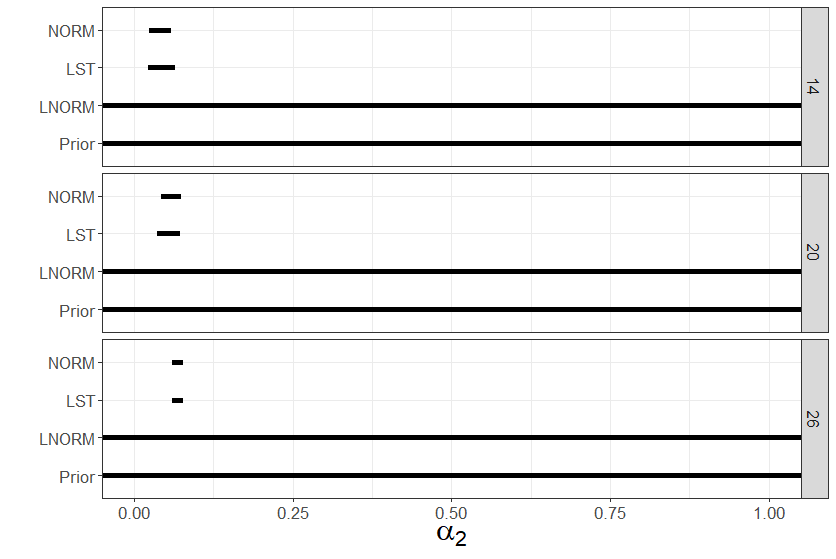
\includegraphics[width=.49\linewidth]{Images/alpha2_post.png}
\end{subfigure}%
\begin{subfigure}
  \centering
  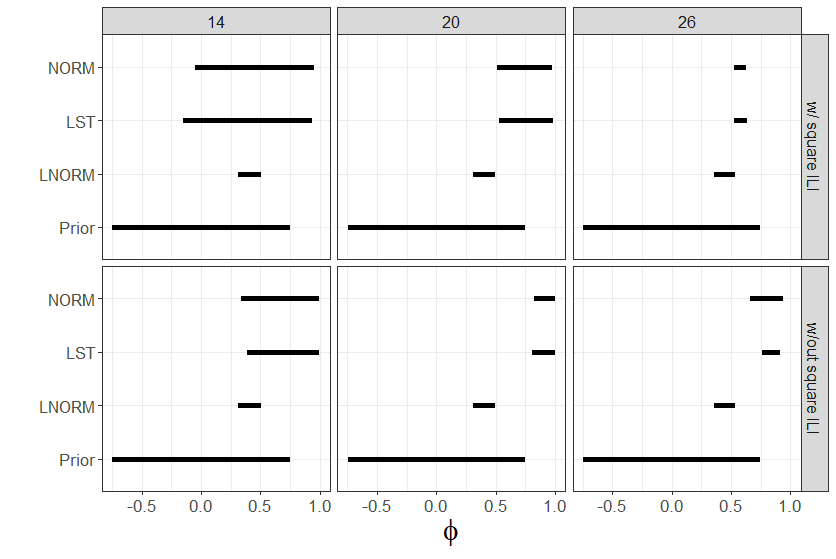
\includegraphics[width=.49\linewidth]{Images/phi_post.png}
\end{subfigure}
\caption{Posterior 95\% credible intervals for $\alpha_0$ for the three hospitalization models separated by whether or not the squared ILI term was included. Intervals are for the US hospitalizations and weeks 14, 20 and 26 are shown (top left). Prior distribution 95\% interval is also included.  95\% posterior credible intervals for $\alpha_1$ for the three hospitalization models separated by whether or not the squared ILI term was included. Intervals are for the US hospitalizations and weeks 14, 20 and 26 are shown (top right). Prior distribution 95\% interval is also included.
95\% posterior credible intervals for $\alpha_2$ for the three hospitalization models. Intervals are for the US hospitalizations and weeks 14, 20 and 26 are shown (bottom left). Prior distribution 95\% interval is also included. 
95\% posterior credible intervals for $\phi$ for the three hospitalization models separated by whether or not the squared ILI term was included (bottom right). Prior distribution 95\% interval is also included. In each plot intervals are for the US hospitalizations and weeks 14, 20 and 26 are shown.}
\label{fig:hosp_lin_params}
\end{figure}


% \begin{figure}[hbt!]
% 
% \begin{subfigure}
%   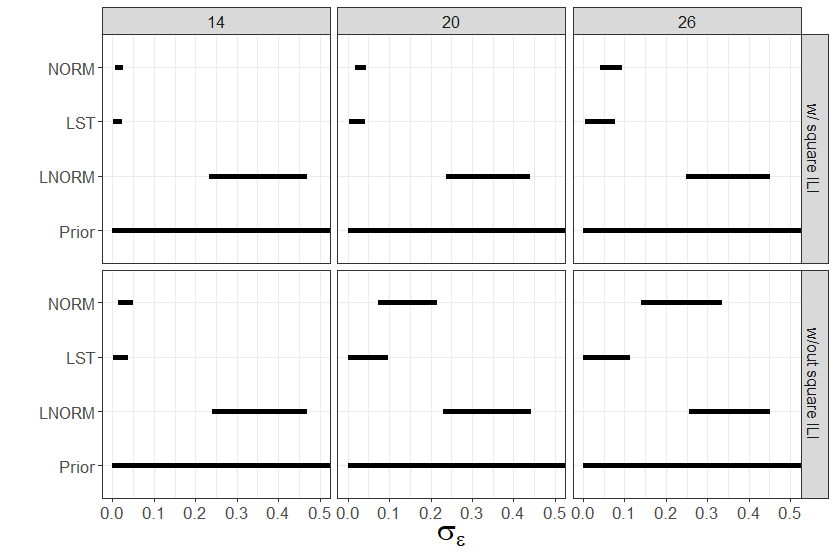
\includegraphics[width=\linewidth]{Images/sigma_epsilon_post.png}
%   % \caption{}
%   % \label{MLEDdet}
% \end{subfigure}\hfill % <-- "\hfill"
% \begin{subfigure}
%   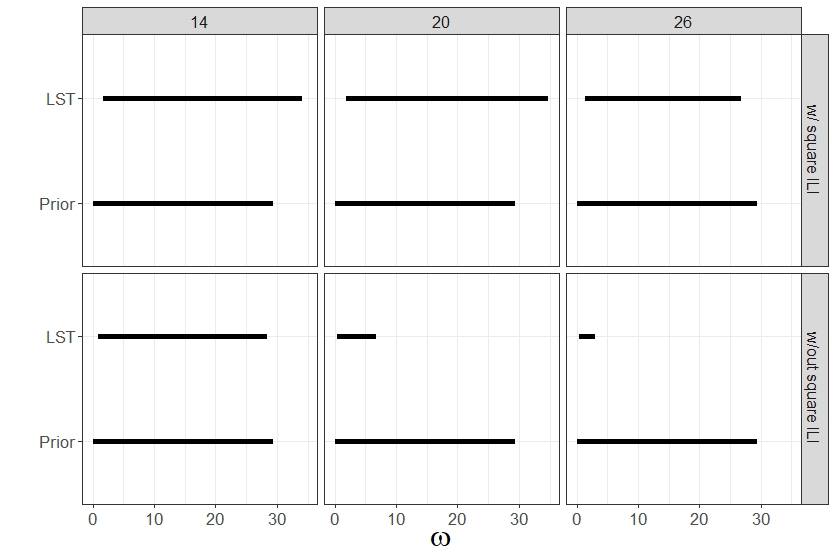
\includegraphics[width=\linewidth]{Images/omega_post.png}
%   % \caption{}
%   % \label{energydetPSK}
% \end{subfigure}
% 
% \caption{Posterior 95\% credible intervals for $\sigma_{\epsilon}$ for hospitalization models with and without the ILI squared term. Intervals are for the US hospitalizations and weeks 14, 20 and 26 are shown (left). Prior distribution 95\% interval is also included.
% 95\% posterior credible intervals for $\omega$ for LST hospitalization models with and without the ILI squared term (right). Prior distribution 95\% interval is also included. In all plots intervals are for the US hospitalizations and weeks 14, 20 and 26 are shown.}
% \label{fig:hosp_nus_param}
% \end{figure}




\begin{figure}[hbt!]
\centering
\begin{subfigure}
  \centering
  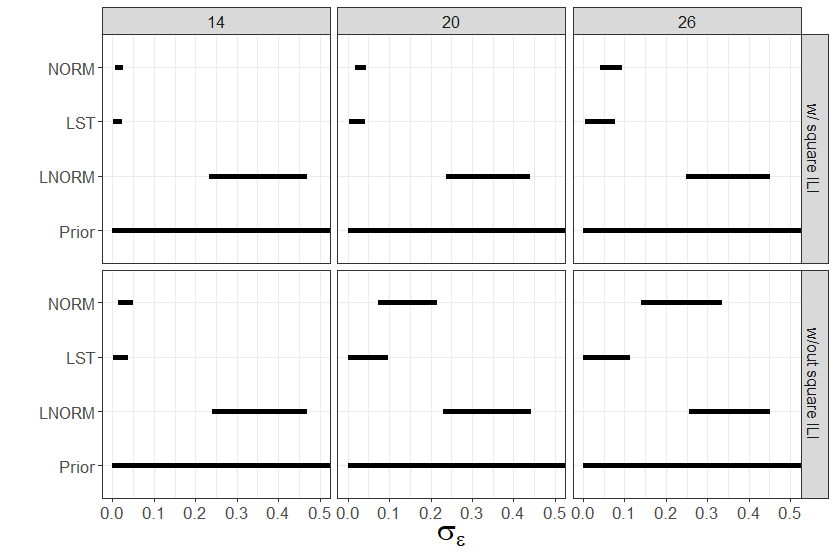
\includegraphics[width=.49\linewidth]{Images/sigma_epsilon_post.png}
  % \caption{95\% posterior credible intervals from ILI model for scale parameter of the model distribution. Shown are intervals from the US model of ILI for weeks 14, 20, and 26. The blue is from the SIR model, purple from SIRD, red from ASG and yellow from ASGD. The green interval is the 95\% interval of the prior distribution.}
  % \label{fig:sub1}
\end{subfigure}%
\begin{subfigure}
  \centering
  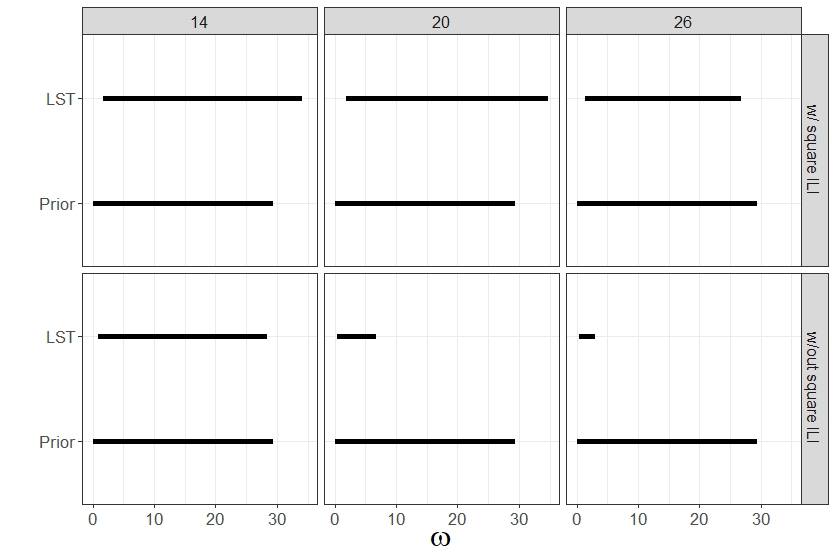
\includegraphics[width=.49\linewidth]{Images/omega_post.png}
  % \caption{95\% posterior credible intervals from ILI model for scale parameter of modeled discrepancy. Shown are intervals from the US model of ILI for weeks 14, 20, and 26. The blue is from the SIRD model and red from ASGD. The green interval is the 95\% interval of the prior distribution.}
  % \label{fig:sub2}
\end{subfigure}
\caption{Posterior 95\% credible intervals for $\sigma_{\epsilon}$ for hospitalization models with and without the ILI squared term. Intervals are for the US hospitalizations and weeks 14, 20 and 26 are shown (left). Prior distribution 95\% interval is also included.
95\% posterior credible intervals for $\omega$ for LST hospitalization models with and without the ILI squared term (right). Prior distribution 95\% interval is also included. In all plots intervals are for the US hospitalizations and weeks 14, 20 and 26 are shown.}
\label{fig:hosp_nus_param}
\end{figure}

\newpage
\section{Model combinations forecast comparison}

We fit 24 forecast models for each location for all 30 weeks, and for each 
week forecast 1-4 week ahead hospitalizations. The 24 models included all 
combinations of ASG, ASGD, SIR, and SIRD ILI models, hospitalization
models where the assumed distribution of 
hospitalizations was normal (NORM), lognormal (LNORM), 
and location-scale t (LST)
hospitalization models, and where ILI was assumed to be a linear or 
quadratic predictor of hospitalizations.

Figure \ref{fig:us_lwis} shows model performance by LWIS for each week of the 
season for all 24 models of US hospitalizations. LWIS scores are grouped by 
ILI model, hospitalization model distribution, and by the linear or quadratic 
modeling. Here, the smaller the LWIS the better. The weeks around the holiday 
week 22 are highlighted by a grey band. 
In several cases, there appears to be a turning point in performance at or 
near week 22. For most ASG models, the models which include discrepancy tend 
to outperform those which do not beginning near week 22 and for the rest of 
the season.
For the SIR models, the discrepancy does not always lead to better forecasts, 
but in for the LNORM hospitalization models, including discrepancy greatly 
improves forecasts around the holiday week 22. The LNORM LWIS scores tend to 
be higher than for LST and NORM hospitalization models, but figure 
\ref{fig:lwis_by_dist_loc} and table \ref{tab:forecast_scores} suggest that 
the LNORM hospitalization model outperforms LST and NORM for most states and 
territories.


\begin{figure}[hbt!]
    
    % \centering
    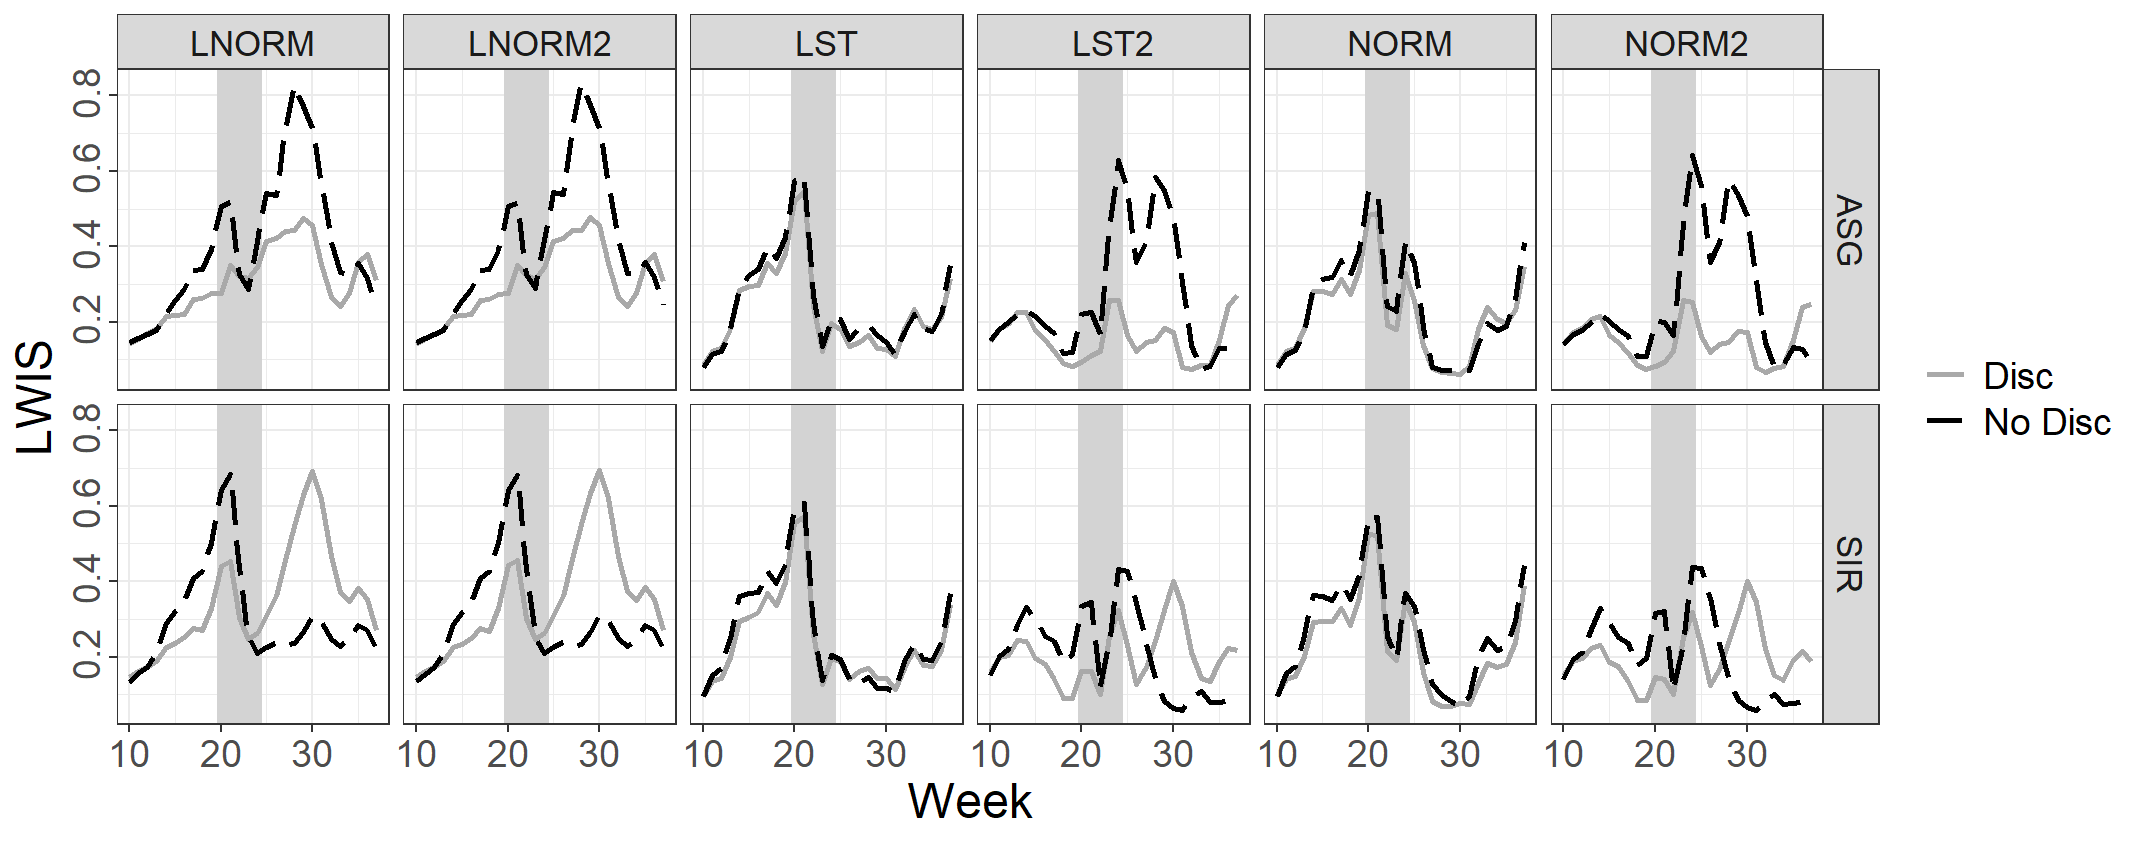
\includegraphics[scale = .5]{Images/lwis_ln_us_full_season.png}
    \caption{Each plot shows the log weighted interval score (LWIS) for every 
    week of the 2023 flu season with scores for models including and exluding 
    discrepancy in the ILI model. Scores are separated by hospitalization 
    distribution family and by ILI as a linear or quadratic predictor. Scores 
    for models with an ASG ILI model are above while those with an SIR model 
    are below. The lower the LWIS the better the forecast.}
    \label{fig:us_lwis}
\end{figure}


Figure \ref{fig:lwis_by_dist_loc} also shows weekly forecast performance by 
LWIS, but all 53 locations are included. The LWIS is shown across the whole 
season faceted by hospitalization model distribution. Overall, the weeks 
leading up to week 22 are the most difficult to forecast, but the LNORM model 
appears to perform the better than the other models during the weeks around 
the holiday week 22. 
The overall LWIS, calculated as the mean LWIS over all locations and weeks, 
for all 
24 models is shown in table \ref{tab:forecast_scores}. The overall best 
performing forecast model combination is ASGD with ILI as a quadratic 
predictor of normally distributed hospitalizations. Forecasts from this 
model combination are compared with forecasts from FluSight in the main text.

In figure \ref{fig:lwis_by_traj_loc}, it appears that both the SIR and ASG 
models which include discrepancy perform better than the models 
which do not include discrepancy.

\begin{figure}[hbt!]
    
    \centering
    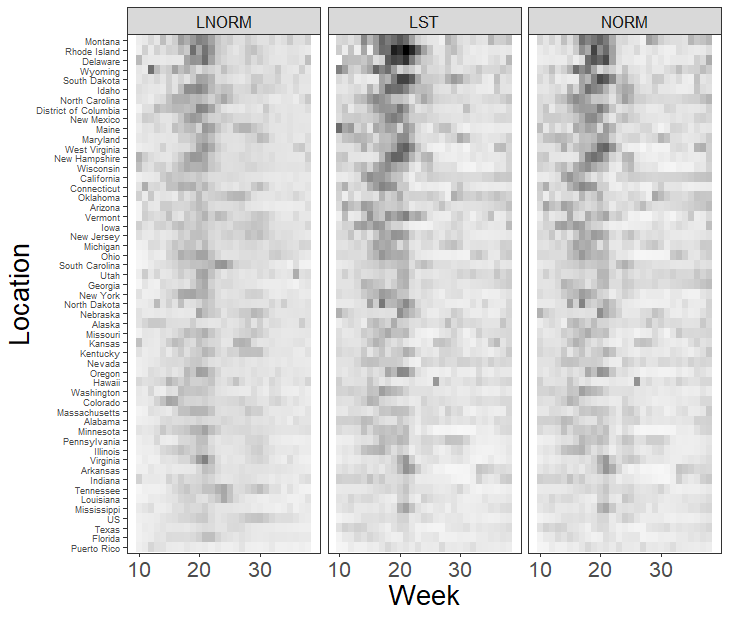
\includegraphics[scale = .6]{Images/lwis_by_dist_loc.png}
    \caption{Each plot shows the log weighted interval scores (LWIS) for all 50 
    US states, PR, DC, and national level forecasts at each week during the 
    2023 flu season. Scores are averaged over all horizons 1-4 weeks ahead. 
    Scores are faceted by hospitalization model distribution. The lighter the 
    shade, the lower the LWIS with low LWIS being better.}
    \label{fig:lwis_by_dist_loc}
\end{figure}




\begin{figure}[hbt!]
    
    \centering
    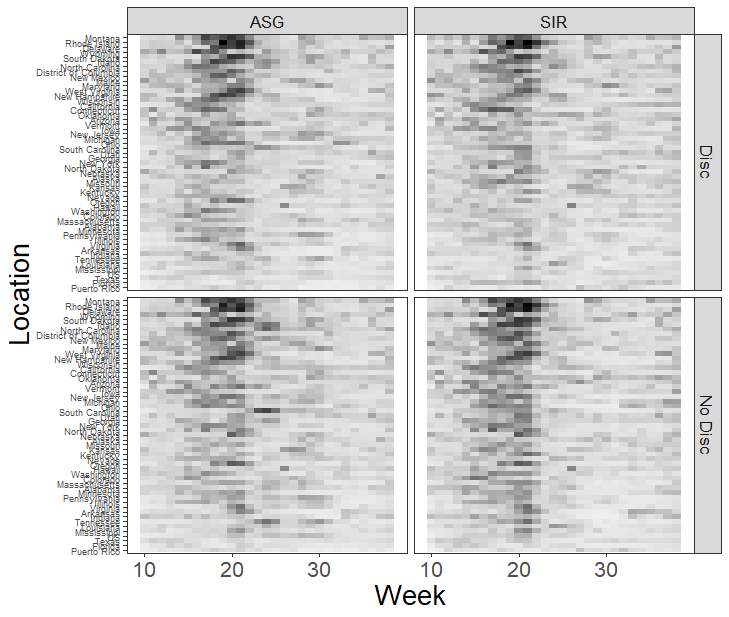
\includegraphics[scale = .7]{Images/lwis_by_traj_loc.png}
    \caption{Each plot shows the log weighted interval scores (LWIS) 
    for all 50 US states, PR, DC, and national level forecasts at each week 
    during the 2023 flu season. Scores are averaged over all horizons 1-4 
    weeks ahead. Scores are faceted by ILI model function (columns) and by 
    whether or not discrepancy modeling was included (rows). The lighter the 
    shade, the lower the LWIS with low LWIS being better.}
    \label{fig:lwis_by_traj_loc}
\end{figure}




\begin{table}
\caption{Overall scores for each of the 24 forecast models. The overall score 
is the log weighted interval score (LWIS) averaged over all locations, weeks, 
and horizons. The scores in the first two rows are for linear models, and the 
scores in the third and fourth rows are for quadratic models. The lowest LWISs 
are bolded.}
\begin{tabular*}{\textwidth}
{@{\extracolsep{\fill}} 
    l*{9}{c}}
  & & \multicolumn{3}{c}{ASG} 
  & \multicolumn{3}{c}{SIR} \\ 
  \cmidrule{3-5} \cmidrule{6-8}
  & & LNORM & LST & NORM & LNORM & LST & NORM\\
  \midrule
  Linear & No Disc & 0.390 & 0.419 & 0.411 & 0.382 & 0.447& 0.442 &\\ 
   & Disc & 0.358 & 0.400 & 0.391 & 0.378 & 0.413 & 0.396 &\\
  \midrule
  Quadratic & No Disc & 0.390 & 0.416 & 0.384 & 0.381 & 0.423 & 0.394 &\\ 
   & Disc & 0.358 & 0.371 & \textbf{0.341} & 0.379 & 0.398 & 0.360 &\\     
  \bottomrule
\end{tabular*}
\label{tab:forecast_scores}
\end{table}






\section{FluSight forecasts WIS comparison}

Figures \ref{fig:wis_cover_sum1} and \ref{fig:state_and_date_wis} are 
similar to figures the main figures in the 2023 flu forecast assessment in the 
main text
except that they show WIS scores instead of LWIS scores. The results of 
foreacst comparison for WIS scores is very similar to those of the LWIS in 
terms of how well the ASGD\_NORM2 forecasts did relative to the others from
the FluSight competition.


\begin{figure}[hbt!]
\begin{adjustwidth}{-1.2cm}{-1.5cm}
    % \begin{minipage}{\linewidth}
    \centering
    \makebox[\linewidth][l]{
    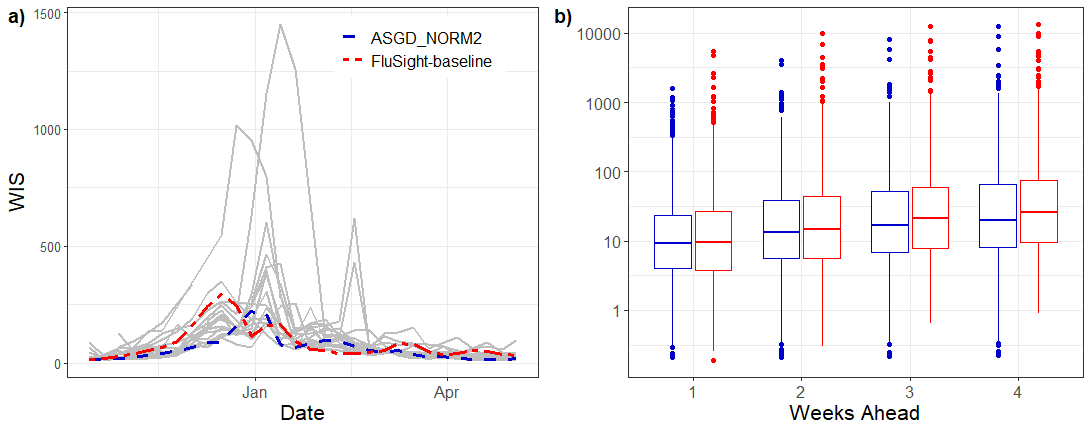
\includegraphics[scale = .54]{Images/wis_cover_sum.png}
    }
    \end{adjustwidth}
    \caption{a) Averaged over location and horizon weighted interval score
    (WIS) for each week during the season for the 21 models being compared.
    Each grey line represents one model, but the ASGD\_NORM2 (blue),
    SIRD\_NORM2 (green), and
    FluSight-baseline (red) are colored to stand out.
    b) Boxplots of all WIS scores for 1, 2, 3, and 4-week ahead horizons
    for the ASGD\_NORM2 (blue), SIRD\_NORM2 (green), and
    FluSight-baseline (red) models.
    To improve vizualization, the $y$-axis
    is on the log scale.}
    \label{fig:wis_cover_sum1}
    % \end{minipage}
    
\end{figure}



\begin{figure}[hbt!]
\begin{adjustwidth}{-1.2cm}{-1.5cm}
    % \begin{minipage}{\linewidth}
    \centering
    \makebox[\linewidth][l]{
    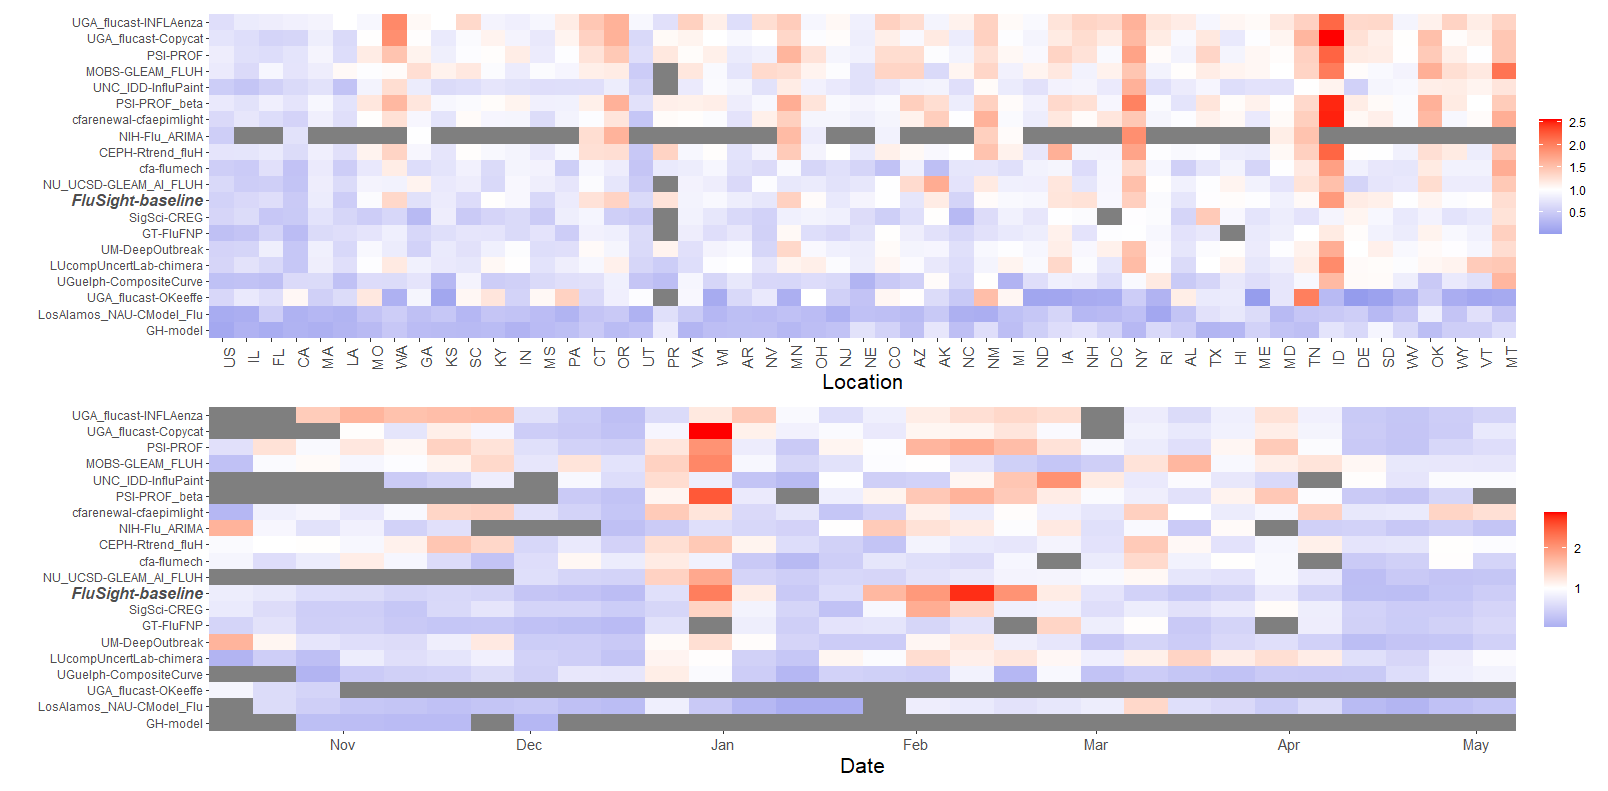
\includegraphics[scale = .5]{Images/state_and_date_wis.png}
    }
    \end{adjustwidth}
    \caption{Ratio of average weighted interval score (WIS) for ASGD\_NORM2 
    to that of each competing FluSight model. Scores are averaged
    over all targets within indicated location (top) or week (bottom) and 
    only include forecasts shared by both models. Lower scores (blue) indicate
    superior performance by the ASGD\_NORM2 model and higher scores (red)
    indicate superior performance by competing model.}
    \label{fig:state_and_date_wis}
    % \end{minipage}
    
\end{figure}

% \begin{figure}[hbt!]
%     \label{fig:wis_cover_sum1}
%     % \centering
%     \begin{adjustwidth}{-1.2cm}{-1.5cm}
%     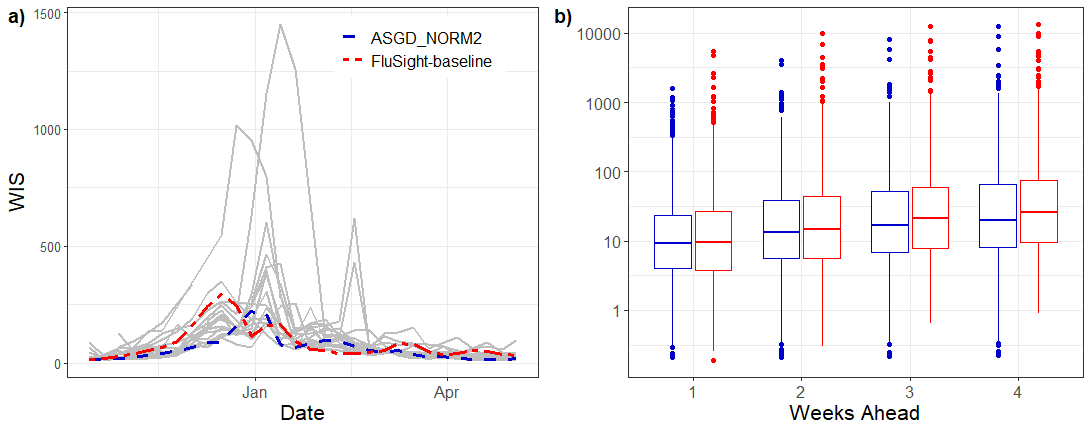
\includegraphics[scale = .54]{Images/wis_cover_sum.png}
%     \caption{a) Averaged over location and horizon weighted interval score
%     (WIS) for each week during the season for the 21 models being compared. 
%     Each grey line represents one model, but the ASGD\_NORM2 (blue),
%     SIRD\_NORM2 (green), and 
%     FluSight-baseline (red) are colored to stand out.
%     b) Boxplots of all WIS scores for 1, 2, 3, and 4-week ahead horizons 
%     for the ASGD\_NORM2 (blue), SIRD\_NORM2 (green), and
%     FluSight-baseline (red) models. 
%     To improve vizualization, the $y$-axis
%     is on the log scale.}
%     \end{adjustwidth}
%     
% \end{figure}






\end{supplement}






\bibliographystyle{ba}
\bibliography{master_bib}

\end{document}

